\section{Clock Class Reference}
\label{classClock}\index{Clock@{Clock}}
{\tt \#include $<$clock.h$>$}

Collaboration diagram for Clock:\nopagebreak
\begin{figure}[H]
\begin{center}
\leavevmode
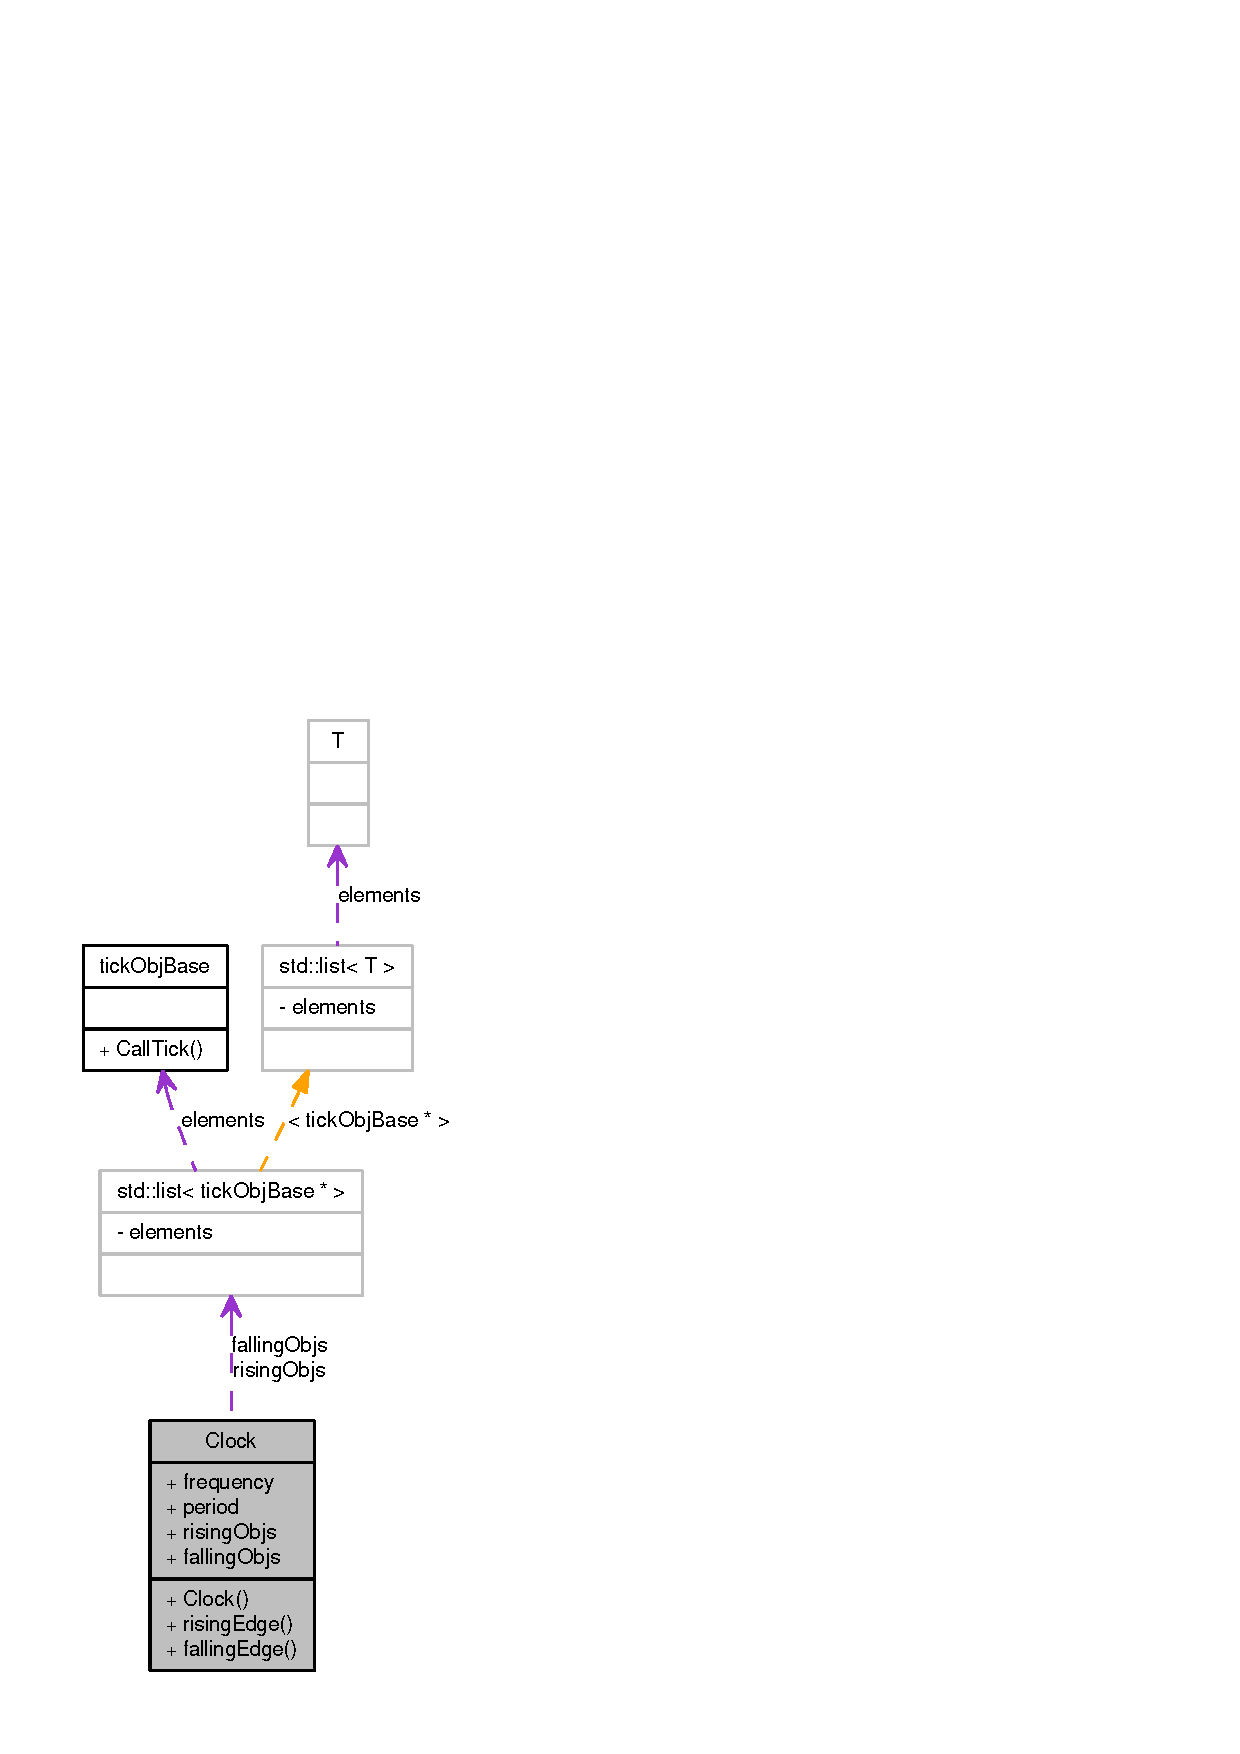
\includegraphics[height=400pt]{classClock__coll__graph}
\end{center}
\end{figure}
\subsection*{Public Member Functions}
\begin{CompactItemize}
\item 
{\bf Clock} (double)
\item 
void {\bf risingEdge} ()
\item 
void {\bf fallingEdge} ()
\end{CompactItemize}
\subsection*{Public Attributes}
\begin{CompactItemize}
\item 
double {\bf frequency}
\item 
double {\bf period}
\item 
list$<$ {\bf tickObjBase} $\ast$ $>$ {\bf risingObjs}
\item 
list$<$ {\bf tickObjBase} $\ast$ $>$ {\bf fallingObjs}
\end{CompactItemize}


\subsection{Detailed Description}


Definition at line 23 of file clock.h.

\subsection{Constructor \& Destructor Documentation}
\index{Clock@{Clock}!Clock@{Clock}}
\index{Clock@{Clock}!Clock@{Clock}}
\subsubsection[{Clock}]{\setlength{\rightskip}{0pt plus 5cm}Clock::Clock (double {\em freq})}\label{classClock_49d7d94582b08b480cfe22f835e5d24b}




Definition at line 7 of file clock.cc.

References fallingEdge(), frequency, Simulator::Now(), period, risingEdge(), and Simulator::Schedule().

\subsection{Member Function Documentation}
\index{Clock@{Clock}!fallingEdge@{fallingEdge}}
\index{fallingEdge@{fallingEdge}!Clock@{Clock}}
\subsubsection[{fallingEdge}]{\setlength{\rightskip}{0pt plus 5cm}void Clock::fallingEdge ()}\label{classClock_c1901911de32ed117b40b6e14168e084}




Definition at line 30 of file clock.cc.

References fallingObjs, Simulator::Now(), period, and Simulator::Schedule().

Referenced by Clock().

Here is the caller graph for this function:\nopagebreak
\begin{figure}[H]
\begin{center}
\leavevmode
\includegraphics[width=124pt]{classClock_c1901911de32ed117b40b6e14168e084_icgraph}
\end{center}
\end{figure}
\index{Clock@{Clock}!risingEdge@{risingEdge}}
\index{risingEdge@{risingEdge}!Clock@{Clock}}
\subsubsection[{risingEdge}]{\setlength{\rightskip}{0pt plus 5cm}void Clock::risingEdge ()}\label{classClock_7e15f1ce4bbe1ee05b1336191086ec30}




Definition at line 18 of file clock.cc.

References Simulator::Now(), period, risingObjs, and Simulator::Schedule().

Referenced by Clock().

Here is the caller graph for this function:\nopagebreak
\begin{figure}[H]
\begin{center}
\leavevmode
\includegraphics[width=123pt]{classClock_7e15f1ce4bbe1ee05b1336191086ec30_icgraph}
\end{center}
\end{figure}


\subsection{Member Data Documentation}
\index{Clock@{Clock}!fallingObjs@{fallingObjs}}
\index{fallingObjs@{fallingObjs}!Clock@{Clock}}
\subsubsection[{fallingObjs}]{\setlength{\rightskip}{0pt plus 5cm}list$<${\bf tickObjBase}$\ast$$>$ {\bf Clock::fallingObjs}}\label{classClock_85868b33b134e520b3512c2130f5244f}




Definition at line 35 of file clock.h.

Referenced by fallingEdge(), and registerClock().\index{Clock@{Clock}!frequency@{frequency}}
\index{frequency@{frequency}!Clock@{Clock}}
\subsubsection[{frequency}]{\setlength{\rightskip}{0pt plus 5cm}double {\bf Clock::frequency}}\label{classClock_d293cfc6a12bf9b6ba204cb3efc2bac4}




Definition at line 28 of file clock.h.

Referenced by Clock().\index{Clock@{Clock}!period@{period}}
\index{period@{period}!Clock@{Clock}}
\subsubsection[{period}]{\setlength{\rightskip}{0pt plus 5cm}double {\bf Clock::period}}\label{classClock_1bff60a169a5db12917207d37358f446}




Definition at line 29 of file clock.h.

Referenced by Clock(), fallingEdge(), and risingEdge().\index{Clock@{Clock}!risingObjs@{risingObjs}}
\index{risingObjs@{risingObjs}!Clock@{Clock}}
\subsubsection[{risingObjs}]{\setlength{\rightskip}{0pt plus 5cm}list$<${\bf tickObjBase}$\ast$$>$ {\bf Clock::risingObjs}}\label{classClock_ed711a85f243ca3f49a403750a5445b9}




Definition at line 33 of file clock.h.

Referenced by registerClock(), and risingEdge().

The documentation for this class was generated from the following files:\begin{CompactItemize}
\item 
{\bf clock.h}\item 
{\bf clock.cc}\end{CompactItemize}
